\chapter{BLOOD VESSEL CHARACTERIZATION USING VIRTUAL 3D MODELS AND CONVOLUTIONAL NEURAL NETWORKS IN FLUORESCENCE MICROSCOPY}
\label{chap:ISBI}

\let\thefootnote\relax\footnotetext{
This chapter previously appeared as:
A. Chowdhury, D.~V. Dylov., Q. Li, M. MacDonald, D.~E. Meyer, M. Marino and A. Santamaria-Pang, "Blood vessel characterization using virtual 3D models and convolutional neural networks in fluorescence microscopy" \emph{IEEE International Symposium on Biomedical Imaging}, pp. 629-632, 2017}

%%% INTRODUCTION
\section{Introduction}

In this chapter of the thesis, we address the problem of minimization of error in image classification by taking the approach of redressing imbalance in datasets using data augmentation techniques. The image pre-processing layer of the image classification pipeline is modified to reduce classification error as shown in Fig. \ref{fig:chapter2}.

\begin{figure}[ht!]
\centering
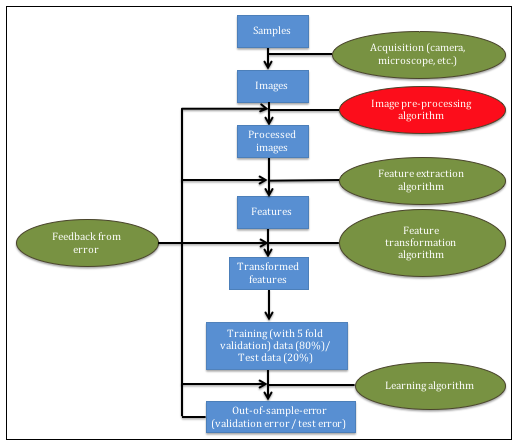
\includegraphics[width=1.0\textwidth]{img/chapter2}
\caption{Reducing classification error by modifying algorithms from the image pre-processing layer of the image classification pipeline. The step highlighted in red is modified for reducing the out of sample error.}
\label{fig:chapter2}
\end{figure}

Specifically, we make parametric 3D models of blood vessel vasculature for balancing the dataset for performing classification between morphologies of blood vessels.
Characterizing the morphology of vasculature in digital pathology is an important step in defining the microenvironment within brain tissue samples. In particular, understanding the geometry of vessel configuration and its changes during a disease may provide deeper insight into the progression of neuropathological degenerative diseases such as Alzheimer\'s disease. Images acquired using 20x object from immunofluorescent (IF) stained 6 um tissue sections with collagen IV antibody are used in this work.  We attempt to characterize three different types of blood vessel morphologies which are found in relative abundance in our image data set. They are singular blood vessels with no visible lumen, singular blood vessels with a distinct lumen and blood vessels appearing as a pair; which we have named \textit{RoundLumen-}, \textit{RoundLumen+}, and \textit{Twins} correspondingly.
In this work, we show that it is possible to characterize blood vessels using convolutional neural networks (CNN) as opposed to traditional image processing techniques which involve segmentation and hand-crafted feature extraction. Instead, here we use pre-trained CNN to extract features from the images. This technique of deep transfer learning is compared to the visual bag of words (VBW) method for feature extraction \cite{yang2007evaluating}. We conclude from the results that the features from pre-trained CNN are able to distinguish the morphologies of blood vessels better than the standard VBW method. 
Additionally, our work also shows that the construction of 3 dimensional (3D) virtual models of vasculature using parametric methods is a promising tool for dealing with infrequent scenarios in vascular analysis of brain tissue section. Acquisition of natural training samples is a time consuming and labor intensive process. Deep learning requires abundant training data for tuning the large number of parameters of the various inherent models. If a certain class is imbalanced then the classification models could become prone to biased outcomes. The construction of 3D parametric models, presented here tackles these issues and creates a balanced high-fidelity classification model. 
In this study, we built a basic 3D vasculature model using our prior knowledge of blood vessel geometry, as guided by a pathologist. The 3D vasculature was repeatedly sliced at various angles and orientations to obtain 2D samples for training the machine learning model, thereby mimicking the physical sectioning of tissue during sample preparation for microscopy. In addition, a filtering technique was then used to fine-tune the virtual data to reflect the variability present in the naturally acquired samples. We train three models based on: virtual data, natural data and a mixture of both. The models are then tested on a reserved, independent portion of the naturally occurring data, with a hierarchical classification being performed to demonstrate a proof of concept. 
The first classification task involves distinguishing between singular blood vessels (\textit{RoundLumen}) and pair of blood vessels (\textit{Twins}). The second task of finer granularity is the classification between \textit{RoundLumen-} and \textit{RoundLumen+}. We report various metrics for both the classification tasks and observe that the artificial data improves upon the model trained from only the natural data.
As far as we know, this is the first attempt to model vasculature using parametric 3D geometric methods exclusively. Statistical 2D and 3D shape models have been used extensively in medical image segmentation as detailed in \cite{heimann2009statistical}. However, these models use the training samples to statistically find a model of the object of interest. We do not generate virtual 2D models because we believe that we can obtain more variability in the training data by sectioning from the 3D models. Additionally, the 3D models may be extended to various other modalities in medical imaging. 

%%% Data
\section{Data}

This section provides a detailed explanation of the different morphologies of blood vessels that are explored in this study. The first subsection is a description of the natural data curated from actual postmortem human tissue samples. The second subsection involves the description of the virtual 3D model of blood vessels which are used for generating samples for training the convolutional neural networks.

\subsection{Natural data}
FFPE Postmortem brain tissue samples from ten subjects with neurological disorders underwent sequential IF-multiplexing and fluorescent imaging. For each subject, approximately 25 images were acquired.   This involves a cycling process of tissue section staining with 2-3 dye-labeled antibodies, imaging, dye inactivation and repeated staining with a new set of dye-labeled antibodies. Images underwent illumination correction, registration, stitching and auto-fluorescence subtraction. Collagen IV was used as a marker to detect all blood vessels. An image overlay is shown in Fig. \ref{fig:morphologies}.

\begin{figure}[ht!]
\centering
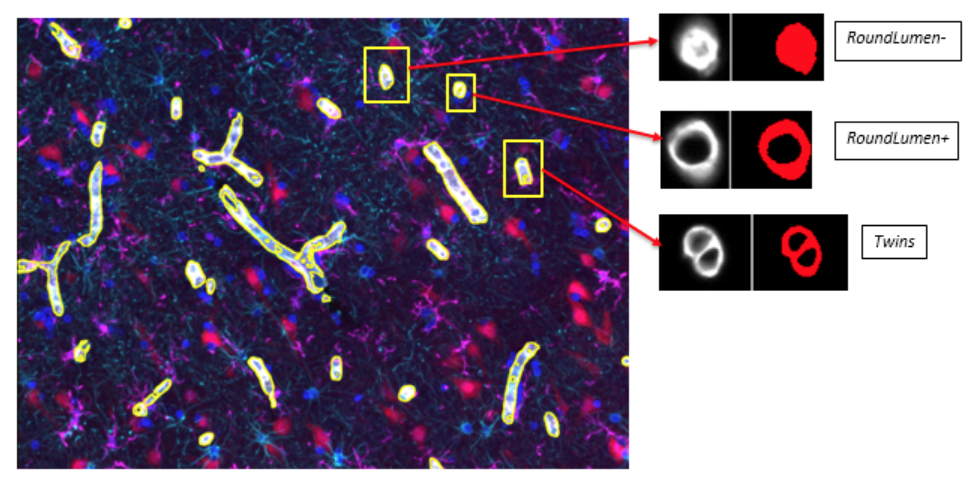
\includegraphics[width=1.0\textwidth]{img/morphologies}
\caption{Depiction of the different morphologies in the natural data with respect to a multichannel image, overlaid with different protein markers. The three types of morphologies analyzed in this study is represented on the right.}
\label{fig:morphologies}
\end{figure}

The number of instances of the three different types of morphologies are depicted in Table \ref{table:classes}.
\begin{table}[ht!]
\caption{Distribution of vascular morphologies}
\centering
\begin{tabular}{ | c | c |} 
\hline
\textit{RoundLumen-} & 689 \\ 
\hline
\textit{Roundlumen+} & 3427 \\ 
\hline
\textit{Twins} & 266 \\ 
\hline
Total & 4382 \\ 
\hline
\end{tabular}
\label{table:classes}
\end{table}

\subsection{Virtual data}
The construction of the artificial model starts with defining a set of control points in three dimensional Cartesian coordinates. The control points reflect the basic structure that the blood vessel is supposed to represent. This is followed by interpolating between the points using a 3D cubic spline interpolator. This forms the skeleton or the center line that represents the center or the lumen of the blood vessel and is shown in Fig. 2(a). The 3D volume of the blood vessel is constructed after this step. We first define a number of parameters; the inner radius of the blood vessel (r); the outer radius (R). The number of sampling points along the spline (N); the number of sampling points in the radial direction (Nr). At each sampling point; we define a circular disk along the z-axis; by randomly perturbing the values of r and R. We also define an intensity model for the blood vessels depicted in Eq. \ref{eq:1}. From the natural images, it seems that the intensity is high in the periphery of the blood vessel and decays towards the lumen and as we move away from the periphery. We model this using an exponential decay in the following form:

\begin{equation}
I(d) = I_{max} \exp(- \alpha |r\prime - d|)
\label{eq:1}
\end{equation}


where, $I_{max}$  is the maximum intensity, is the calibration coefficient (in mm-1 units), $r\prime=(R+r)/2.$ $d$ is the distance from the center of the lumen. At each point on the disc, we define the voxel density as a normal distribution with mean $I(d)$ and standard deviation 0.01. This is followed by formulating the rotation matrix by calculating the angle between the tangent to the spline at that sampling point and the z-axis. The points corresponding to each point on the disc are therefore mapped or rotated along the curve by multiplying the coordinates with the rotation matrix. An example of this rotation is depicted in Fig. \ref{fig:3D_model}(b). We then discretize the coordinates such that we obtain an actual 3D image in the form of an array. This is depicted in Fig. \ref{fig:3D_model}(c). The intensity values are normalized and assigned to the corresponding discretized points in the 3-dimensional array. The volume rendered version of the 3D image is depicted in Fig. \ref{fig:3D_model}(d). Therefore, by changing the parameters of the model we can build several different 3D images and slice it at various angles to mimic the natural tissue cross sections at various depths and angles. Some examples the various models are depicted in Fig. \ref{fig:slicer}.

\begin{figure}[ht!]
\centering
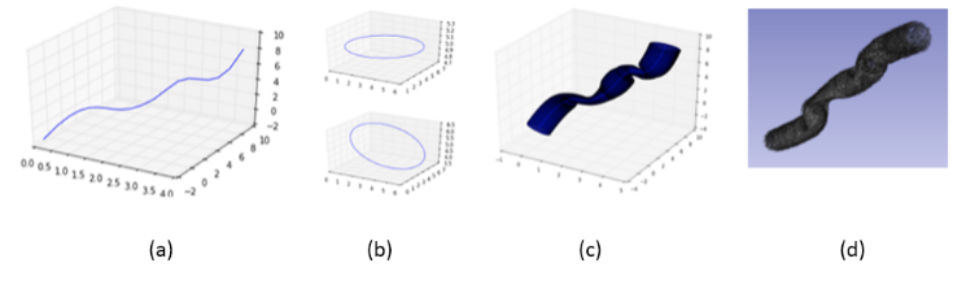
\includegraphics[width=1.0\textwidth]{img/3D_model}
\caption{Development of the 3D virtual model}
\label{fig:3D_model}
\end{figure}

\begin{figure}[ht!]
\centering
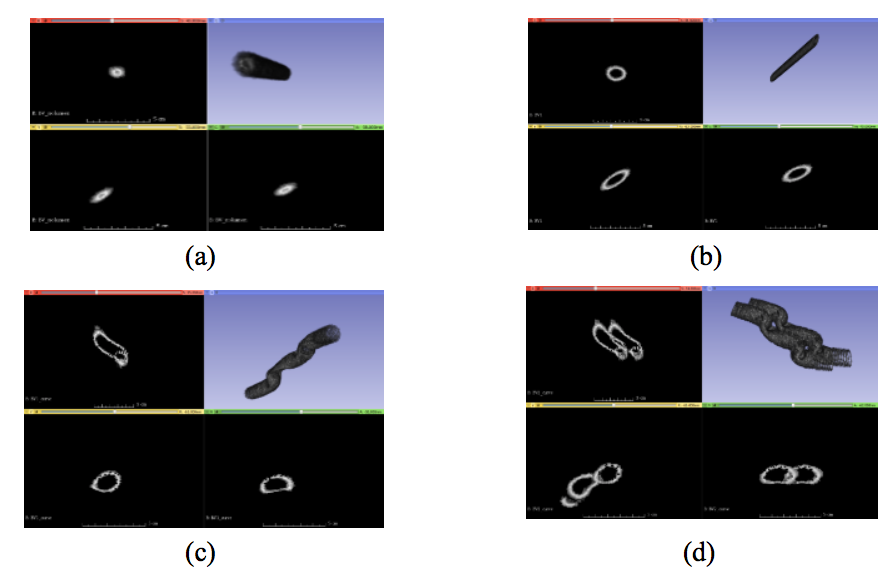
\includegraphics[width=1.0\textwidth]{img/slicer}
\caption{3D virtual models and their corresponding projections along different planes of view (a) Linear model of \textit{RoundLumen-} (b) Linear model of \textit{RoundLumen+} (c) Non-linear model of \textit{RoundLumen+} (d) Non-linear model of \textit{Twins}}
\label{fig:slicer}
\end{figure}

The process of construction of the different types of morphologies in blood vessels is the same as that explained above. Fig.  \ref{fig:slicer}(a) is a blood vessel with a no lumen (\textit{RoundLumen-}) and a linear skeleton. The control points are chosen such that they lie on the major diagonal of the unit cube; i.e. on the line x=y=z in Cartesian coordinates.  Figures  \ref{fig:slicer}(b) and  \ref{fig:slicer}(c) are blood vessel with a single lumen having linear and non-linear structures respectively. Fig.  \ref{fig:slicer}(d) is a model of a \textit{Twin}. As we can see from the cross-sectional views, we obtain different types of morphologies that are similar to actual morphologies in the natural images. A very simple way of creating these multi-vessel structures is by perturbing or shifting the sampling points of the skeleton along a random direction. For example; to come up with a model of \textit{RoundLumen-}, we simply set the inner radius r to 0. As shown in Fig. 3; the different morphologies that commonly occur naturally can be generated. As explained in the introduction; this serves as a viable alternative to using natural data for training convolutional networks.

\section{Methods}

A convolutional neural network is a type of artificial neural network in which are inspired by the organization of the 
animal visual cortex. CNNs consist of multiple neuron collections which process portions of the input image called receptive fields. The outputs are then tiled so that the input regions overlap and this in turn produces a better representation of the original image. This is what makes CNNs translation invariant. 
The CNN is made up of four types of layers: the input layer, the convolutional layer, the non-linear layer, the pooling layer; and the fully connected layer. The input layer is where the networks accept the images.  The images consist of raw pixel values depicted by width, height and the number of channels.  The convolutional layer will compute the output of the neurons that are connected to local regions in the input, each computing a dot product between their weights and a receptive field. The non-linear layer is the activation function responsible for introducing the non-linearity in the model. The various types of non-linear functions include the sigmoid, the tanh, and the rectified linear unit. The pooling layer performs a down sampling operation. The high-level reasoning in the neural network is done by fully connected layers.  Their activations can be performed by simple matrix multiplication.
In this work, we use the pre-trained convolutional neural networks as a feature extractor. This network consists of weights trained on the ImageNet dataset. We extract the 6th layer in the network which is a 4096-dimensional vector as a representation of the image. This may be considered as a transfer learning model because we transfer the weights learnt from another domain to blood vessel recognition. We use a pre-trained neural network called AlexNet \cite{krizhevsky2012imagenet} to extract features from the data. 

We perform an experiment to show that pre-trained CNNs are efficient in representing the vascular morphology. The experiment is performed on the natural data where 33 \% of the data is held out as test data and the rest is used for training. Two models are developed. One of them uses the visual bag of words (VBW) \cite{yang2007evaluating} feature extraction method to extract the features; the other uses the AlexNet architecture to extract the features. A three-class classification (one vs rest) is performed using the logistic regression classifier. The accuracy, f1-score, precision and recall calculated on the same test data are reported for comparison.

\begin{table}[ht!]
\centering
\caption{Comparison of feature extraction methodologies}
\begin{tabular}{ | c | c | c | c | c |} 
\hline
Feature extractor  & Accuracy	& f1-score	 & Precision & Recall \\ 
\hline
\textit{AlexNet} & 91.92 & 91.93 & 91.98 & 91.92 \\ 
\hline
\textit{VBW} & 78.38	& 77.38 & 	76.71 & 78.38 \\
\hline
\end{tabular}
\label{table:FE}
\end{table}

The results in Table \ref{table:FE} show that pre-trained convolutional neural networks are a good choice for representation of vascular morphology.

\section{Experiments and results}
Features are extracted using the AlexNet architecture which is trained on the ImageNet \cite{deng2009imagenet} database. The weight parameters are used to extract the features in a feedforward manner. This is called transfer learning. 33 \% of the natural data is held out as test data. All the experiments are performed on this dataset for maintaining consistency in the results. 
A filtering technique is introduced to appropriately extract slices from the 3D volumes. This is done by obtaining the probabilities of the artificial data using a model trained on the natural training data. The probabilities of the corresponding images are then sorted and the images with the highest probabilities are selected. This is a way to boost the artificial model.  The filtered virtual data is then used to retrain the classifier. Examples of both the natural and artificial data are represented in the Fig. \ref{fig:slices}.

\begin{figure}[ht!]
\centering
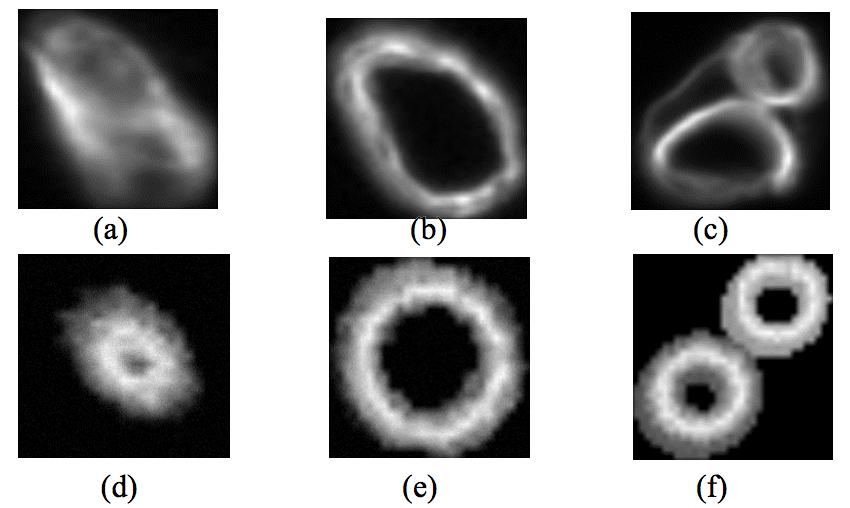
\includegraphics[width=1.0\textwidth]{img/slices}
\caption{ Examples of vessel classes \textit{RoundLumen-} (a/d), \textit{RoundLumen+} (b/e) and \textit{Twins} (c/f) for natural (a/b/c) and virtual data (d/e/f)}
\label{fig:slices}
\end{figure}

A hierarchical classification is performed to first classify the single blood vessels from blood vessels that bundled in pairs i.e \textit{RoundLumen} vs \textit{Twins}. The second classification task involves distinguishing between \textit{RoundLumen-} and \textit{RoundLumen+}. We perform three different types of training to demonstrate our proposed methods. The first type of training is done with only the naturally occurring data. The second type of training data consists only of the artificial data that has been filtered by the natural model as explained before. Finally, the third type consists of both the artificial and natural training samples. We refer to this as Mixed. All the results are reported on the held out 33 \% of the natural data. The accuracy, f1-score, precision, recall and receiver operating characteristic (ROC), and precision-recall (PR) curves are reported in the following tables and figures for each of the two classification tasks. 

\begin{table}[ht!]
\centering
\caption{Results of binary classification between \textit{RoundLumen} and \textit{Twin}}
\begin{tabular}{ | c | c | c | c | c |} 
\hline
Data & Accuracy & f1-score & Precision & Recall \\ 
\hline
\textit{Artificial} & 92.81& 59.36	& 45.24 & \textbf{86.36} \\ 
\hline
\textit{Natural} & 96.34& 71.03& 68.42& 73.86 \\
\hline
\textit{Mixed} & \textbf{97.71} & \textbf{81.76} & \textbf{79.57} & 84.01 \\
\hline
\end{tabular}
\label{table:results}
\end{table}


\begin{figure}[ht!]
    \centering
    \begin{subfigure}[t]{0.5\textwidth}
     \centering
       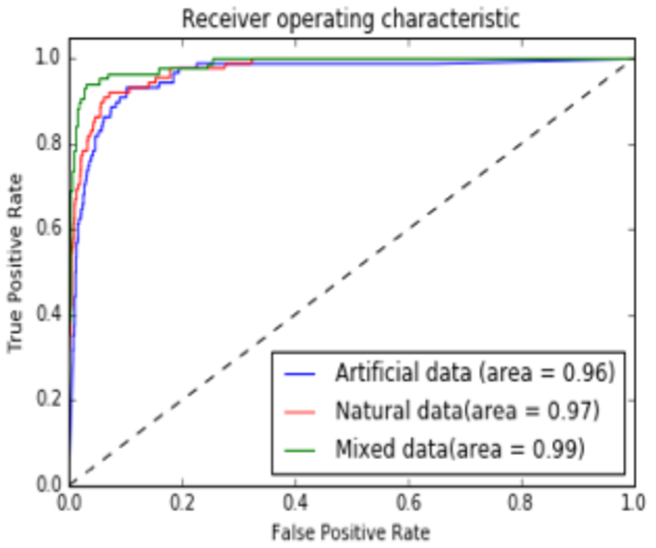
\includegraphics[width=1.0\linewidth]{img/single_twins_ROC.pdf}
  \caption{ROC curve}
        \label{fig:ROC1}   
    \end{subfigure}%
    \begin{subfigure}[t]{0.5\textwidth}
        \centering
          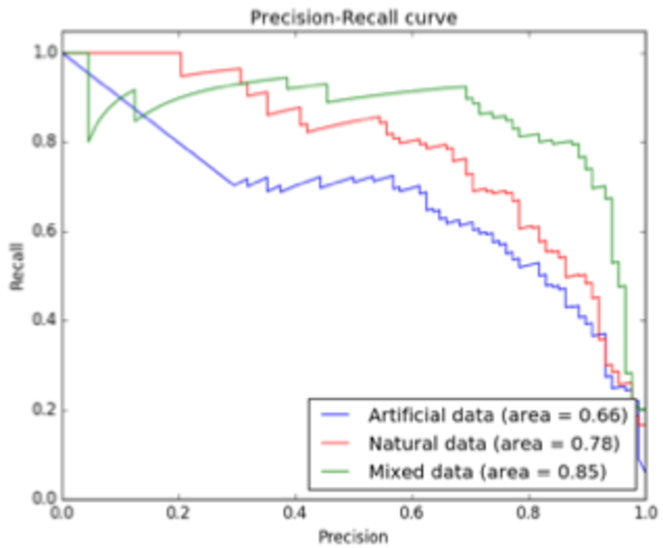
\includegraphics[width=1.0\linewidth]{img/single_twins_PRC.pdf}
  \caption{PR curve }
        \label{fig:PRC1}
    \end{subfigure}%
    \caption{Plots of the receiver operating characteristics (ROC) curve and the precision recall (PR) curve of the classification between \textit{RoundLumen} and \textit{Twins} along with the area under the curves (AUC) for the three experiments denoted as legends in the plots. From the nature of the curves, and the values of the AUC, we conclude that combining the using \textit{mixed} data performs better than using the \textit{Natural} data or the \textit{Artificial data} in isolation.}
    \label{fig:ROC_PRC1}
\end{figure}


\begin{table}[ht!]
\centering
\caption{Results of binary classification between \textit{RoundLumen-} and \textit{RoundLumen+}}
\begin{tabular}{ | c | c | c | c | c |} 
\hline
Data & Accuracy & f1-score & Precision & Recall \\ 
\hline
\textit{Artificial} & 98.38 & 99.02 & 99.38 & 98.67 \\ 
\hline
\textit{Natural} & 96.34& 71.03& 68.42& 73.86 \\
\hline
\textit{Mixed} & \textbf{98.60} &  \textbf{99.16} & \textbf{99.29} & \textbf{99.03} \\
\hline
\end{tabular}
\label{table:results1}
\end{table}


\begin{figure}[ht!]
    \centering
    \begin{subfigure}[t]{0.5\textwidth}
     \centering
       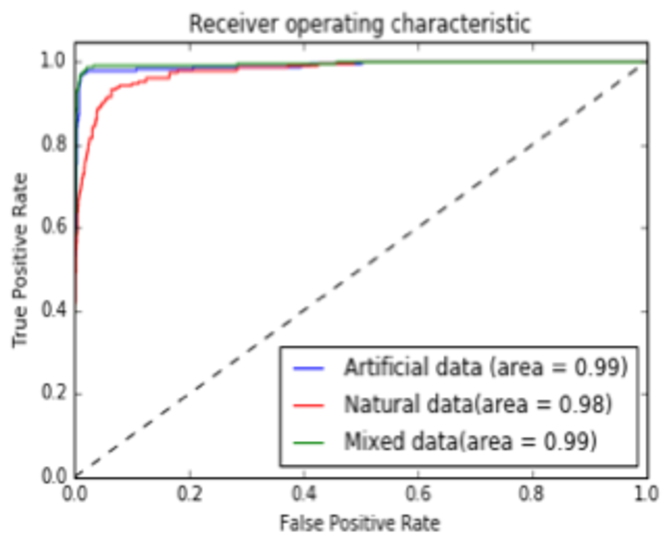
\includegraphics[width=1.0\linewidth]{img/roundlumens_ROC.pdf}
  \caption{ROC curve}
        \label{fig:ROC2}   
    \end{subfigure}%
    \begin{subfigure}[t]{0.5\textwidth}
       \centering
          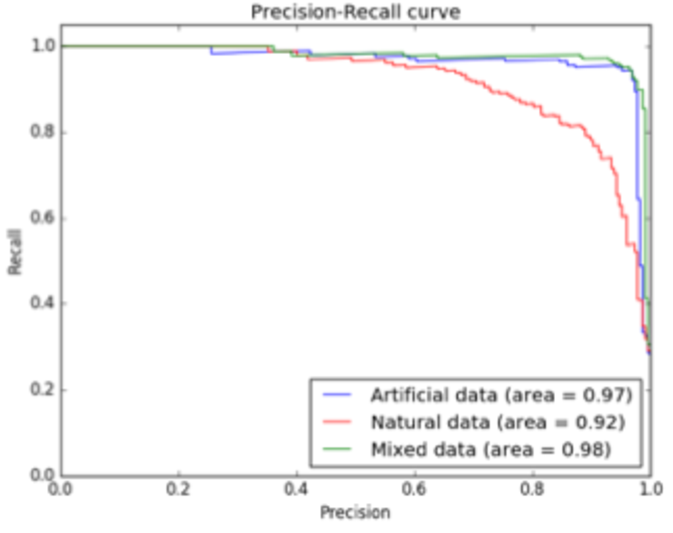
\includegraphics[width=1.0\linewidth]{img/roundlumens_PRC.pdf}
  \caption{PR curve }
        \label{fig:PRC2}
    \end{subfigure}%
    \caption{Plots of the receiver operating characteristics (ROC) curve and the precision recall (PR) curve of the classification between \textit{RoundLumen+} and \textit{RoundLumen-} along with the area under the curves (AUC) for the three experiments denoted as legends in the plots. From the nature of the curves, and the values of the AUC, we conclude that combining the using \textit{mixed} data performs better than using the \textit{Natural} data or the \textit{Artificial data} in isolation.}
    \label{fig:ROC_PRC2}
\end{figure}

The ROC and PR curves are calculated using the minority class in both the classification tasks, i.e. \textit{Twins} for the first classification task and \textit{RoundLumen-} for the second task.
From Table \ref{table:results}, we can see that the artificial data captures the differences between the two classes. It is also able to identify \textit{Twins}, which is the minority class in Task 1, from the high recall. Therefore, the results are boosted when we combine both the artificial and natural data. In addition, the ROC and PR curves in Figs. \ref{fig:ROC_PRC1} confirms our hypothesis that virtual data may be used for building the models. The naturally trained model performs better than the virtual trained model. However, as we can see from the ROC curves, the model built from the mixed data improves the performance. Table \ref{table:results1} and Fig.  \ref{fig:ROC_PRC2} presents the corresponding results for the second classification task. In this case, we see that the virtual data performs better than the natural data and boosts the performance when trained on its own or in union with the natural data.

\section{Conclusions}
We have shown that the use of deep learning algorithms  trained with a mixture of virtual and natural data  results in a more accurate prediction of vasculature morphologies than the use of standard feature extraction methods (such as visual bag of words). The methodology of complementing natural data with synthetic samples holds potential for becoming a standard approach in deep learning with unbalanced datasets. In neuroscience, it could be applied to help elucidate the underlying mechanisms of common neurological degenerative diseases.
This work shows how we can use artificial parametric 3D models to perform data augmentation for characterizing morphologies of blood vessels. This chapter therefore shows how the choice of algorithms in every component of the image classification pipeline is so important for minimizing the error in the image classification problem. In the next part of the thesis, we demonstrate how to quantify the error from different components of the image classification pipeline.